\documentclass[final]{beamer}

\usepackage[scale=1.24]{beamerposter} % Use the beamerposter package for laying out the poster

\usetheme{confposter} % Use the confposter theme supplied with this template

\setbeamercolor{block title}{fg=black,bg=white} % Colors of the block titles
\setbeamercolor{block body}{fg=black,bg=white} % Colors of the body of blocks
\setbeamercolor{block alerted title}{fg=white,bg=black} % Colors of the highlighted block titles
\setbeamercolor{block alerted body}{fg=black,bg=white} % Colors of the body of highlighted blocks
% Many more colors are available for use in beamerthemeconfposter.sty

%-----------------------------------------------------------
% Define the column widths and overall poster size
% To set effective sepwid, onecolwid and twocolwid values, first choose how many columns you want and how much separation you want between columns
% In this template, the separation width chosen is 0.024 of the paper width and a 4-column layout
% onecolwid should therefore be (1-(# of columns+1)*sepwid)/# of columns e.g. (1-(4+1)*0.024)/4 = 0.22
% Set twocolwid to be (2*onecolwid)+sepwid = 0.464
% Set threecolwid to be (3*onecolwid)+2*sepwid = 0.708

\newlength{\sepwid}
\newlength{\onecolwid}
\newlength{\twocolwid}
\newlength{\threecolwid}
\setlength{\paperwidth}{48in} % A0 width: 46.8in
\setlength{\paperheight}{36in} % A0 height: 33.1in
\setlength{\sepwid}{0.024\paperwidth} % Separation width (white space) between columns
\setlength{\onecolwid}{0.22\paperwidth} % Width of one column
\setlength{\twocolwid}{0.464\paperwidth} % Width of two columns
\setlength{\threecolwid}{0.708\paperwidth} % Width of three columns
\setlength{\topmargin}{-0.5in} % Reduce the top margin size
%-----------------------------------------------------------

\usepackage{graphicx}  % Required for including images

\usepackage{booktabs} % Top and bottom rules for tables

%----------------------------------------------------------------------------------------
%	TITLE SECTION 
%----------------------------------------------------------------------------------------

\title{Champernowne Constant} % Poster title

\author{Abhishek Rajput} % Author(s)

\institute{Department of Computer Science and Software Engineering\\ [1.0ex]
\vspace*{1.5ex}
		   SOEN 6481: SOFTWARE SYSTEMS REQUIREMENTS SPECIFICATION} % Institution(s)
		   

%----------------------------------------------------------------------------------------

\begin{document}

\addtobeamertemplate{block end}{}{\vspace*{2ex}} % White space under blocks
\addtobeamertemplate{block alerted end}{}{\vspace*{2ex}} % White space under highlighted (alert) blocks

\setlength{\belowcaptionskip}{2ex} % White space under figures
\setlength\belowdisplayshortskip{2ex} % White space under equations

\begin{frame}[t] % The whole poster is enclosed in one beamer frame

\begin{columns}[t] % The whole poster consists of three major columns, the second of which is split into two columns twice - the [t] option aligns each column's content to the top

\begin{column}{\sepwid}\end{column} % Empty spacer column

\begin{column}{\onecolwid} % The first column

%----------------------------------------------------------------------------------------
%	OBJECTIVES
%----------------------------------------------------------------------------------------

\setbeamercolor{block alerted title}{fg=white,bg=brown} % Change the alert block title colors
\setbeamercolor{block alerted body}{fg=black,bg=white} % Change the alert block body colors

\begin{alertblock}{Objectives}
\begin{itemize}
\item To familiarize the audience with Champernowne constant.
\item To share my learnings and challenges faced during the course of the project.
\item To give an overview of the calculator developed as a part of this project.  
\end{itemize}

\end{alertblock}

%----------------------------------------------------------------------------------------
%	INTRODUCTION
%----------------------------------------------------------------------------------------
\vspace{3cm}
\begin{block}{Introduction}

\textbf{Champernowne Constant (C\textsubscript{10})}

\begin{itemize}
\item Named after economist and mathematician D. G. Champernowne.
\item Is a transcendental real constant whose decimal expansion has important properties.
\item For base 10, this number is a normal number.
\item This constant is interesting because any given sequence of numbers can be shown to exist somewhere in the Champernowne representation.
\end{itemize}

\end{block}
\vspace{1.5cm}
%------------------------------------------------

\begin{figure}
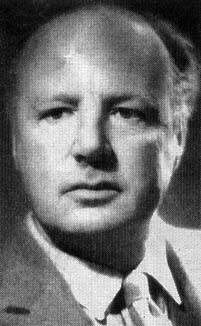
\includegraphics[width=16cm, height=20cm]{DGChampernowne.jpg}
\caption{David Gawen Champernowne, 1912-2000}
\end{figure}

%----------------------------------------------------------------------------------------

\end{column} % End of the first column

\begin{column}{\sepwid}\end{column} % Empty spacer column

\begin{column}{\twocolwid} % Begin a column which is two columns wide (column 2)

\begin{columns}[t,totalwidth=\twocolwid] % Split up the two columns wide column

\begin{column}{\onecolwid}\vspace{-.6in} % The first column within column 2 (column 2.1)

%----------------------------------------------------------------------------------------
%	CALCULATOR
%----------------------------------------------------------------------------------------

\begin{block}{Calculator}

\textbf{Overview}

\begin{itemize}
\item Used for generating Champernowne Constant to given decimal places based on the users' input.
\item Could also be used for performing basic mathematical calculations on positive numbers.
\item Developed in Java using Swing (GUI) widget toolkit.
\end{itemize}

\vskip3cm

\textbf{Key Functionalities}

\begin{itemize}
\item Generating Champernowne Constant.
\item Calculating the position of the first occurrence of a given number in the generated Champernowne Constant.
\item Calculating the total number of occurrences of a given number in the generated Champernowne Constant.
\item Retrieving the last generated Champernowne Constant in the input field to perform basic calculations.
\end{itemize}

\vskip3cm

\textbf{User Interface} \\
\vspace{0.7cm}
 The UI of the calculator includes:

\begin{itemize}
\item Output screen
\item Input field
\item Number and Operation keys
\item Instruction screen
\end{itemize}

\end{block}

%----------------------------------------------------------------------------------------

\end{column} % End of column 2.1

\begin{column}{\onecolwid}\vspace{-.6in} % The second column within column 2 (column 2.2)

%----------------------------------------------------------------------------------------
%	METHODS
%----------------------------------------------------------------------------------------
%----------------------------------------------------------------------------------------
%	DID YOU KNOW?
%----------------------------------------------------------------------------------------

\setbeamercolor{block alerted title}{fg=black,bg=dalblue} % Change the alert block title colors
\setbeamercolor{block alerted body}{fg=black,bg=white} % Change the alert block body colors

\begin{alertblock}{Did you know?}

Champernowne's Constant fooled early programs meant to check if certain sequences of numbers were truly random. \newline
The programs searched to see if each one-digit number, two-digit number, three-digit number and so on showed up as often as it should have if the numbers were truly random, and they did.

\end{alertblock}

\vspace{2cm}
%------------------------------------------------

\begin{figure}
\fbox{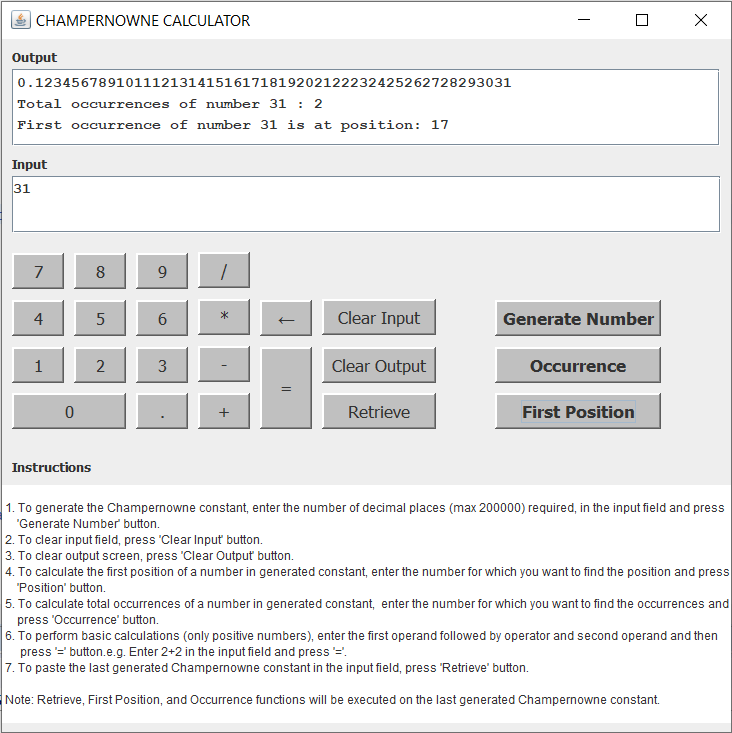
\includegraphics[width=25cm, height=30cm]{calculator.PNG}}
\caption{Champernowne Calculator}
\end{figure}

%----------------------------------------------------------------------------------------
\vspace{2cm}


\end{column} % End of column 2.2

\end{columns} % End of the split of column 2 - any content after this will now take up 2 columns width

%----------------------------------------------------------------------------------------
%	IMPORTANT RESULT
%----------------------------------------------------------------------------------------

\setbeamercolor{block alerted title}{fg=black,bg=dalgold} % Change the alert block title colors
\setbeamercolor{block alerted body}{fg=black,bg=white} % Change the alert block body colors

\begin{alertblock}{Champernowne Constant}
For base 10, the number is defined by concatenating representations of successive integers.
\[ \textbf{C\textsubscript{10} = 0.12345678910111213141516...} \]

\end{alertblock} 

%----------------------------------------------------------------------------------------

\end{column} % End of the second column

\begin{column}{\sepwid}\end{column} % Empty spacer column

\begin{column}{\onecolwid} % The third column

%----------------------------------------------------------------------------------------
%	CHALLENGES
%----------------------------------------------------------------------------------------

\begin{block}{Challenges}

\begin{itemize}
\item Learning Latex and proper usage of packages.
\item Preparing good questionnaires for interviews was a time-consuming process.
\item Difficulties faced while scheduling interviews because of the time difference between India and Canada.
\item Embedding persona template in Latex code was a bit challenging.
\item Finding out extend and include relationships was a slightly intricate task.
\end{itemize}

\end{block}

%----------------------------------------------------------------------------------------
%	LEARNINGS
%----------------------------------------------------------------------------------------

\begin{block}{Learnings}

\begin{itemize}
\item Insightful knowledge about Champernowne Constant.
\item Learned about transcendental numbers and normal numbers.
\item Hands-on experience of Latex code.
\item Significant improvements in documentation skills.
\item Defining target users for our envisioned end product in Persona.
\item Gained knowledge on how to document project artifacts for the envisioned end product.
\item Practical implementation of different project artifacts like Domain Model, Use Case model, User Stories, etc.
\end{itemize}

\end{block}



\vspace{5cm}
\begin{center}

\includegraphics[width=0.8\linewidth]{Concordia-University-logo.png}
\end{center}
%----------------------------------------------------------------------------------------

\end{column} % End of the third column

\end{columns} % End of all the columns in the poster

\end{frame} % End of the enclosing frame

\end{document}
